\chapter{Soldering}

\section{Overview}

If you're going to do any electronics work, you're going to have to do some soldering. Many people fear it before they've done it, but it's really pretty simple to do. This exercise will show you how to solder a DC power connector to a set of wires for a breadboard.

\subsection{Parts}

To do it, you'll need:

\begin{figure}[!htb]
     \centering
     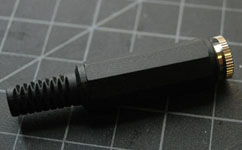
\includegraphics[scale=0.3]{img/soldering/power_connector.jpg}
     \caption{DC Power Jack}
     \label{DC Power Jack}
\end{figure}

\begin{figure}[!htb]
     \centering
     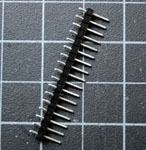
\includegraphics[scale=0.3]{img/soldering/headers.jpg}
     \caption{Header Pins}
     \label{Header Pins}
\end{figure}

\begin{figure}[!htb]
     \centering
     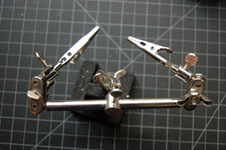
\includegraphics[scale=0.3]{img/soldering/helping_hands.jpg}
     \caption{Helping Hands}
     \label{Helping Hands}
\end{figure}

\begin{figure}[!htb]
     \centering
     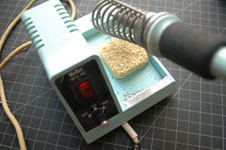
\includegraphics[scale=0.3]{img/soldering/soldering_iron.jpg}
     \caption{Soldering Iron}
     \label{Soldering Iron}
\end{figure}

\begin{figure}[!htb]
     \centering
     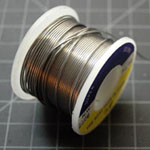
\includegraphics[scale=0.3]{img/soldering/solder.jpg}
     \caption{Solder}
     \label{Solder}
\end{figure}

\begin{figure}[!htb]
     \centering
     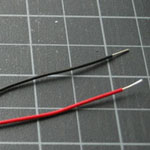
\includegraphics[scale=0.3]{img/soldering/hookup_wire.jpg}
     \caption{22-AWG hookup wire, in red and black}
     \label{22-AWG hookup wire, in red and black}
\end{figure}

\begin{figure}[!htb]
     \centering
     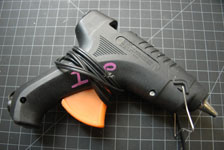
\includegraphics[scale=0.3]{img/soldering/hot_glue_gun.jpg}
     \caption{Hot Glue Gun and Hot Glue}
     \label{Hot Glue Gun and Hot Glue}
\end{figure}

\begin{figure}[!htb]
     \centering
     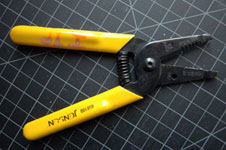
\includegraphics[scale=0.3]{img/soldering/wire_strippers.jpg}
     \caption{Wire Strippers}
     \label{Wire Strippers}
\end{figure}

\subsection{Preparing the parts}

Cut a red and a black wire about four inches in length. Strip the ends back about 1/4 of an inch. Bend a hook on one end of each wire. Unscrew the power jack. Connect the red wire to hole in the the center tab of the power, and the black to the hole in the outside tab. Use pliers to crimp the hooked wires to their connections on the jack. If the connections aren't soldered, you'll get an inconsistent connection at best, and a short circuit at worst.

\begin{figure}[!htb]
     \centering
     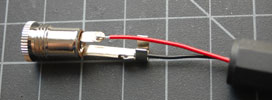
\includegraphics[scale=0.8]{img/soldering/power_connector_unsoldered.jpg}
     \caption{power connector unsoldered}
     \label{power connector unsoldered}
\end{figure}

\subsection{Soldering}

Touch the iron to the joint between the wire and the metal to heat the joint. Then touch the solder to the joint (NOT to the iron) until it melts. This should make a clean solder with a small blob of solder. Twist the wires together and thread them through the sleeve of the jack.

\begin{figure}[!htb]
     \centering
     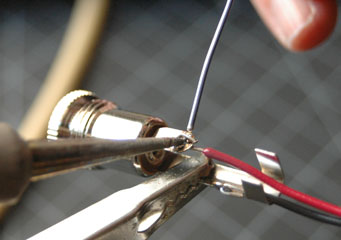
\includegraphics[scale=0.8]{img/soldering/soldering_power_connector.jpg}
     \caption{soldering power connector}
     \label{soldering power connector}
\end{figure}

The result should look like this:

\begin{figure}[!htb]
     \centering
     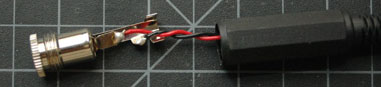
\includegraphics[scale=2.5]{img/soldering/power_conn_inside.jpg}
     \caption{power connector inside}
     \label{power connector inside}
\end{figure}


Trim the ends of the wires to the same length, and strip them back to about 1/8th of an inch. Break off two header pins and hold them in one clip of the helping hands. Clip the wires in the other clip, and align them with the header pins like so:

\begin{figure}[!htb]
     \centering
     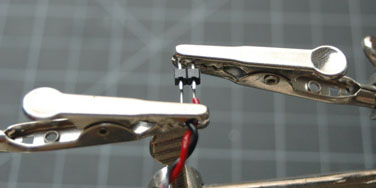
\includegraphics[scale=2.5]{img/soldering/soldering_headers.jpg}
     \caption{soldering headers}
     \label{LEDs}
\end{figure}

When you're done soldering, you should have two separate blobs like this:

\begin{figure}[!htb]
     \centering
     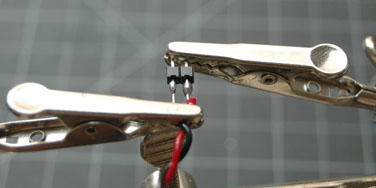
\includegraphics[scale=2.5]{img/soldering/soldering_headers_2.jpg}
     \caption{soldering headers 2}
     \label{soldering headers 2}
\end{figure}



If you can't see space between the two solder joints, de-solder them and do it again. You need to be sure there's no connection between these wires that can cause a short circuit, and the best way to do that is to leave space.
Take a hot glue gun and surround the bare connections to protect them and provide some strain relief. When you're done, you should have a connection like this:

\begin{figure}[!htb]
     \centering
     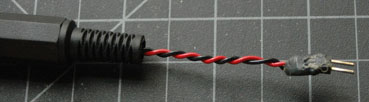
\includegraphics[scale=2.5]{img/soldering/power_conn_headers.jpg}
     \caption{power connector headers}
     \label{power connector headers}
\end{figure}

Make sure you can tell which pin is connected to the red wire and which is connected to the black.

\subsection{Testing}

Before you connect it to power, take a meter and check the connections for continuity. The center pin should be connected to the red wire, and the outer rim should be connected to black. When that's good, you're ready to use it.
